 % COMAP2024SCUT template
 % Created by Caibin Zeng, email: macbzeng@scut.edu.cn  %
 % January 8, 2025
 %%
 
 %美赛模板:正文部分

 \documentclass[12pt]{article}  % 官方要求字号不小于 12 号,此处选择 12 号字体
 % \linespread{1.1}
 % \bibliographystyle{plain}
 % 本模板不需要填写年份,以当前电脑时间自动生成
 %%%%%%%%%%%%%%%%%%%%%%%%%%%%%%%%%%%%%%%%%%%%%%%%%%%%%%%%%%%%%%%%%%%%%%%%%%%%%%%
 % 请在以下的方括号中填写队伍控制号
 \usepackage[2511654]{easymcm}  % 载入 EasyMCM 模板文件
 \problem{B}  % 请在此处填写题号
 %%%%%%%%%%%%%%%%%%%%%%%%%%%%%%%%%%%%%%%%%%%%%%%%%%%%%%%%%%%%%%%%%%%%%%%%%%%%%%%%
 % \usepackage{mathptmx}  % 这是 Times 字体,中规中矩 
 \usepackage{palatino}  % mathpazo 这palatino是 COMAP 官方杂志采用的更好看的 Palatino 字体,可替代以上的 mathptmx 宏包
 \usepackage{ctex}
 \usepackage{pdfpages}
 \usepackage{longtable}
 \usepackage{tabu}
 \usepackage{threeparttable}
 \usepackage{listings}
 \usepackage{paralist}
 \usepackage{hyperref}
 \usepackage[linesnumbered,ruled,vlined]{algorithm2e}
 \usepackage{subfigure}
 \usepackage{subcaption}
 \usepackage{cleveref} %可以调用
 \usepackage{tcolorbox}
 \usepackage{amsmath}
 \tcbuselibrary{most}
 \newtcolorbox{mybox}[2][]{colbacktitle=red!10!white, colback=blue!10!white,coltitle=red!70!black, title={#2},fonttitle=\bfseries,#1}
 \graphicspath{{img/}}          % 此处{img/}为相对路径,注意加上“/”
  \let\itemize\compactitem
  \let\enditemize\endcompactitem
 \newcommand{\upcite}[1]{\textsuperscript{\textsuperscript{\cite{#1}}}}
 
 
 \title{Sustain the happiness of everyone:\\ A Multi-objective Optimization Model for Juneau Tourism}  % 标题
 
 % 如需要修改题头(默认为 MCM/ICM),请使用以下命令(此处修改为 MCM)
 %\renewcommand{\contest}{MCM}
 
  %文档开始
 \begin{document}
 
 % 此处填写摘要内容
 \begin{abstract}
Juneau City in Alaska, USA is facing the problem of overtourism. The number of tourists and tax rates need to be adjusted to improve the satisfaction of tourists and residents, and finally realize sustainable development of tourism industry. The government has implemented some measures to limit the number of tourists, protect the environment, and improve local infrastructure, but the results have not been satisfactory due to the complex factors affecting tourist and resident satisfaction.
     
This article establishes a new satisfaction evaluation model that comprehensively considers the impact of tourist numbers on residents' income, government spending, ecological environment, and social pressure, in order to adjust the daily number of tourists and achieve multi-objective optimization of tourist and resident satisfaction.

\textit{The main steps are as follows:}
 
First, a causal model was established to analyze the principle of how the number of tourists affects tourist satisfaction and resident satisfaction.

 Then, based on the causal model and combined with the searched data, several equations were established to construct a multi-objective optimization model for the impact of tourist numbers on tourist satisfaction and resident satisfaction.

 To maximize stakeholder satisfaction, the NSGA-II genetic algorithm is used to solve the Pareto solution of the multi-objective problem and determine the optimal number of tourists.
 
 This study successfully simulated and optimized the number of tourists in Juneau city by constructing a causal diagram model, which benefits both tourists and residents, and more importantly, can achieve sustainable development of tourism in the Juneau area. In addition, through adjustments, the model can be applied to other destinations affected by excessive tourism and has good universality.
     
 % 此处填写关键字,以分号分开
     \vspace{5pt}  %mm	毫米	1 mm = 2.845 pt   pt 点	1 pt = 0.351 mm
     \textbf{Keywords}: Causal Model; Overtourism; Multi-objective optimization; NSGA-II; Sustainable tourism;
 
 \end{abstract}
 
 \maketitle  % 生成 Summary Sheet
 
 \tableofcontents  % 生成目录
 
 
 % 正文开始
 % Chapter 1: Introduction
 \section{Introduction}
 \subsection{Background}
In recent years, the rapid development of the global tourism industry has brought many challenges, among which the problem of overtourism is particularly prominent. Take Juneau, Alaska, USA as an example. The city received about 1.6 million cruise passengers in 2023, setting a new record. On the busiest days of the tourism season, Juneau could receive up to seven large cruise ships, with as many as 20,000 visitors. Although these tourists brought in a substantial revenue of about 375 million dollars for the city, they also caused many problems, such as increased pressure on local infrastructure, tight drinking water supply, difficult waste management, and increased carbon footprint. In addition, overtourism has also had a negative impact on local culture and natural landscapes, of which the recession of Mendenhall Glacier is a typical case. Since 2007, the glacier has receded the equivalent of eight football fields, which not only caused local residents to worry about the disappearance of the glacier, but also raised questions about the sustainability of tourism. Therefore, how to maintain the economic benefits of tourism while reducing its negative impact on the environment and society, and achieve sustainable development, has become an urgent problem for Juneau to solve.
 
 \subsection{Restatement of the Problem}
 Given the context of overtourism in Juneau, Alaska, and its implications on both the environment and local community, the following issues need to be addressed:
 \begin{itemize}
    \item[$\bullet$]Develop a sustainable tourism model for Juneau, considering factors such as visitor numbers, overall revenue, and tourism stabilization measures. Clearly identify the factors to be optimized and those serving as constraints. Include a financial plan for additional revenue and demonstrate its feedback loop into the model for sustainable tourism promotion. Conduct a sensitivity analysis to highlight the most critical factors.
    \item[$\bullet$]Adapt the model to other overtourism-affected destinations, considering how location choice impacts the importance of different measures. Explore ways to use the model to promote less-visited attractions or locations to achieve a balanced tourism distribution.
    \item[$\bullet$]Draft a one-page memo to the Juneau Tourist Council, outlining predictions, the effects of various measures, and recommendations for optimizing outcomes.
 \end{itemize}
\subsection{Our Work}
 
To demonstrate our workflow visually, the flow chart is shown. 
\ref{fig1}.
  

 \begin{figure}[h]  %h此处,t页顶,b页底,p独立一页,浮动体出现的位置 [H]
 
 \centering  %图表居中
 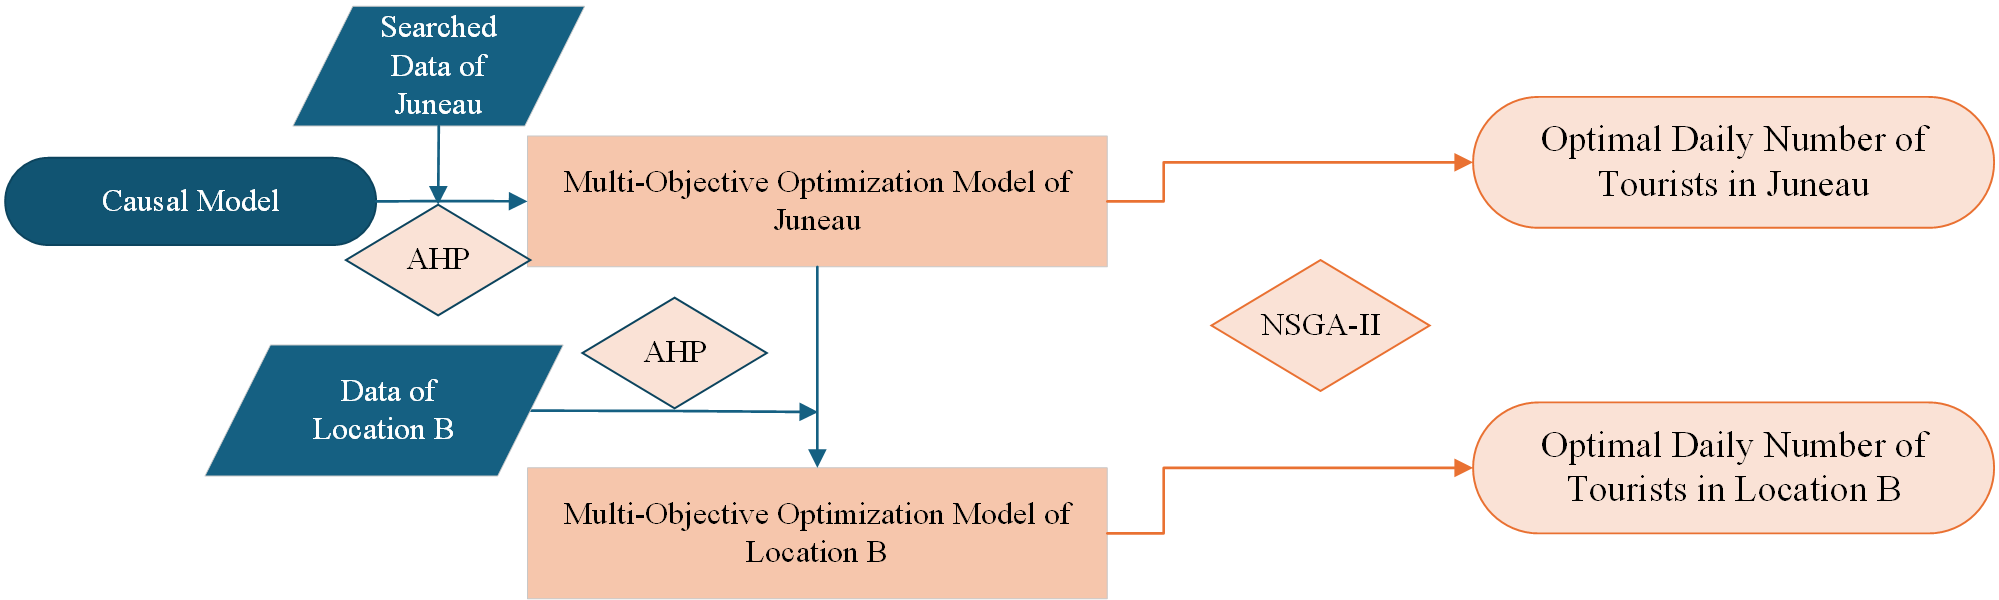
\includegraphics[width=.9\textwidth]{chart2.png} %图片的名称或者路径之中有空格会出问题 
 \caption{Flow Chart of Our Work} % 图片标题                 
 \label{fig1}%交互引用
 \end{figure}
 
 
 \section{Assumptions and Explanations}
 
Since there're several unacquirable data, we simplify our model by making assumptions.
 
 \begin{itemize}
     \setlength{\parsep}{0ex} %段落间距
     \setlength{\topsep}{2ex} %列表到上下文的垂直距离
     \setlength{\itemsep}{1ex} %条目间距
     \item[\bfseries \textit{Assumption} 1:] All the tourists who went to Juneau had been on a cruise.
     %\item[\bfseries \textit{Explanation:}]  
     \vspace{1ex}
     \item[\bfseries \textit{Assumption} 2:] After deducting government expenses from taxes, the remaining funds are all used for infrastructure maintenance and environmental protection.
     %\item[\bfseries \textit{Explanation:}]  XXX
     \vspace{1ex}
     \item[\bfseries \textit{Assumption} 3:] Incorporate all other taxes into the consumption tax rate calculation uniformly.
     %\item[\bfseries \textit{Explanation:}]  XXX
     \vspace{1ex}
     \item[\bfseries \textit{Assumption} 4:] Juneau's revenue comes entirely from the tourism industry.
 \end{itemize}
 
 Additional assumptions are made to simplify the analysis for individual sections. These assumptions will be discussed at the appropriate locations.
 \clearpage
 \section{Notations}
 Some important mathematical notations used in this paper are listed in Table \ref{tab1}. 
 \begin{table}[H]
 \begin{center}
 \caption{Notations used in this paper}
 \begin{tabular}{cc} % 第一列居中对齐、第二列居左对齐
 \toprule[2pt]
 \multicolumn{1}{m{4cm}}{\centering Symbol}
 &\multicolumn{1}{m{10cm}}{\centering Description}\\  %3cm 和 8cm 是列宽,根据实际需求修改
 \midrule
 $x$   &         Tax rate \\
 $T$   &         Tax \\
 $C$   &         Tourists count per year\\
 $E$   &         Consumption per tourist \\
 $TTI$ &         Tax used to maintain infrastructures\\
 $CDI$ &         Each tourist s damagement to infrastructures\\
 $IS$  &         State of infrastructures\\
 $CTS$ &         Tourist\textquotesingle s satisfaction affected by tourist count\\
 $CIS$ &         Tourist\textquotesingle s satisfaction influenced by infrastructures\\
 $LinS$ &        The Locals\textquotesingle satisfaction affected by income\\
 $LIS$ &         The Locals\textquotesingle satisfaction affected by infrastructures\\
 $LS$ &          Satisfaction of the locals\\
 $CS$ &          Satisfaction of the tourists\\
 $Inc$ &         Incomes of each family\\
 $EIE$ &         Expenditure in maintaining infrastructures and environment\\
 $THF$ &         Tourism heat footprint \\
 $wTHF$ &        The whole tourism heat footprint \\
 $\alpha$ &      Loss coefficient of glacier mass balance\\
 $GM$ &          The melting of glacier  \\
 \bottomrule[2pt]
 \end{tabular}	\label{tab1} % 交互引用 
  \iffalse\begin{tablenotes}
         \footnotesize
         \item[*] *\href{https://www.caam.rice.edu/~heinken/latex/symbols.pdf}{ \LaTeX~Mathematical symbols collected by Prof. M. Heinkenschloss}. %此处加入注释*信息
       \end{tablenotes}
       \fi
 \end{center}
 \end{table} 
 \vspace{-1cm} 
 
 
 
 \section{A causal model of the impact of tourist numbers on satisfaction}
 \subsection{Construction of causal model}
 In Juneau, the impacts of tourist count can be simplified into the following model. In order to better quantify the impact of various factors on the locals and tourists, we set tourist satisfaction and local satisfaction as measuring standards.
 
 \begin{figure}[htbp]  %h此处,t页顶,b页底,p独立一页,浮动体出现的位置 [H]
 
    \centering  %图表居中
    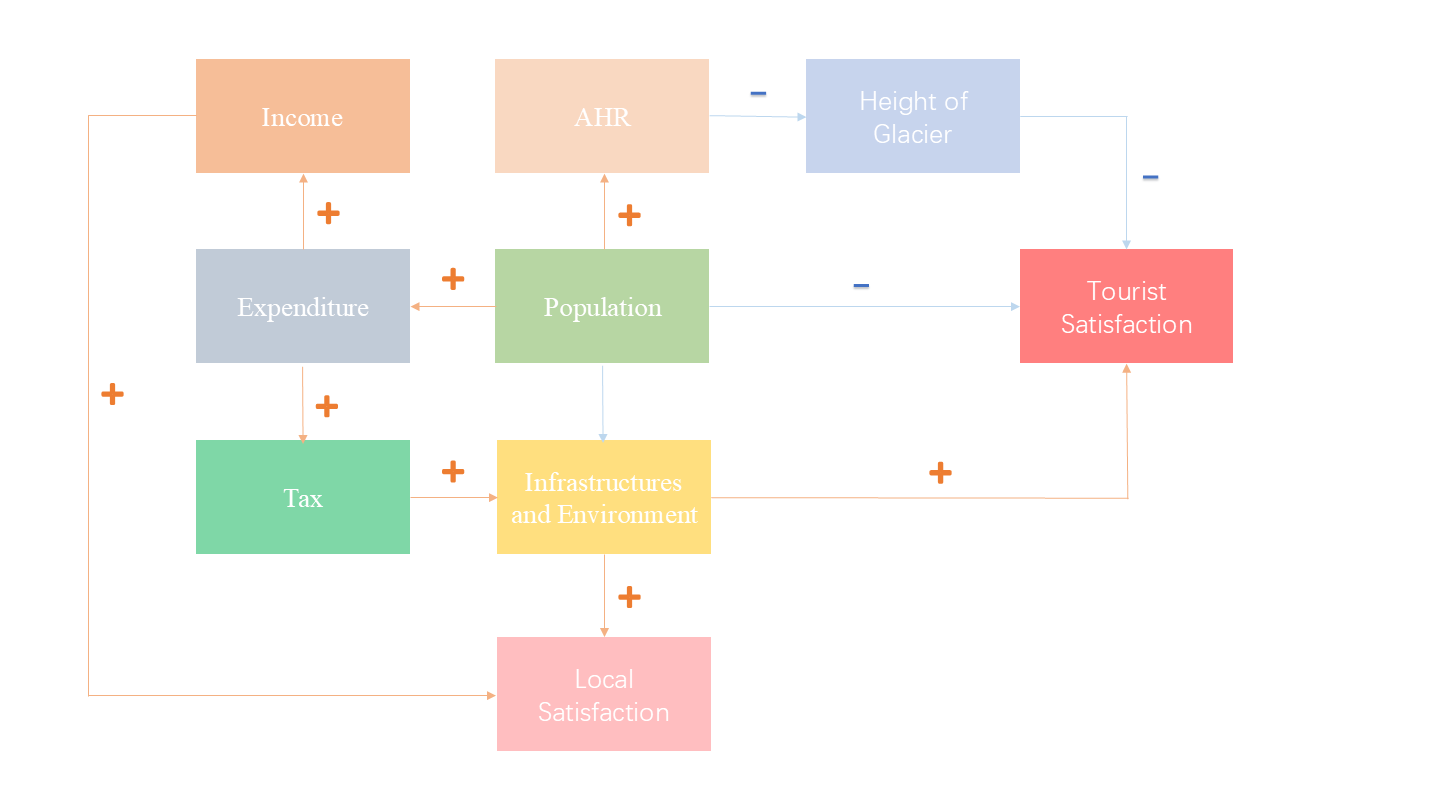
\includegraphics[width=1.2\textwidth]{chart1.png} %图片的名称或者路径之中有空格会出问题 
    \caption{Causal Model of Tourism and Attractions} % 图片标题                 
    \label{fig1}%交互引用
    \end{figure}
 

 \begin{itemize}
     \setlength{\parsep}{0ex} %段落间距
     \setlength{\topsep}{2ex} %列表到上下文的垂直距离
     \setlength{\itemsep}{1ex} %条目间距
 \item [\textbf{Explanations:}] 
        \item Tourist count: The number of tourists. When the number up to a limited point, it will reduce the satisfaction of tourists since its overcrowded experience.
        \item Infrastructures and Environment: The state of infrastructures and the living condition. Overtourism may lead to a considerable deterioration on infrastructures in Juneau and damage on the environment.
        \item Expenditure: The expenditure of tourists, which can be divided into incomes of the locals and taxes. Part of the tax can be used to maintain infrastructures.
        \item AHR: Anthropogenic heat release.
        \item "+": Positive correlation.
        \item "-": Negative correlation.\\
 \end{itemize}
 \subsection{Model Analysis}
 The model is established with reference to literature related to Juneau and objectively analyzes the impacts of different factors. In Figure 2, positive and negative signs are used to indicate the positive and negative correlations between factors. Surveys in Juneau show that an excessive number of tourists can, on the one hand, increase the income of local residents, and on the other hand, put pressure on infrastructure and the environment. However, the increase in the number of tourists can also bring considerable tax revenue to the government, which can be used to maintain infrastructure and carry out environmental construction. On the other hand, through the calculation method of THF (tourism heat footprint), we can calculate the average AHR (Anthropogenic heat release) of tourists, and then predict the glacier melting through AHR. Glacier melting may also lead to a decrease in tourist satisfaction, and the destruction of the environment and infrastructure will simultaneously reduce the satisfaction of both local residents and tourists. Therefore, by using a multi-objective optimization model with the number of tourists as the independent variable, we can obtain the Pareto optimal solution set, and the tourist count within the solution set is relatively ideal and can develop sustainable tourism.
 \subsection{Establishment of mathematical models}
 \begin{enumerate}[(1)]
    \setlength{\parsep}{0ex} %段落间距
\setlength{\topsep}{2ex} %列表到上下文的垂直距离
\setlength{\itemsep}{1ex} %条目间距
\item Mathematical model of tax rate and tourist count\\
The increase in tourism tax will to some extent affect the number of tourists. According to the literature \cite{taxandtour}, we can conclude that for every 10\% increase in tourism tax, the number of tourists will decrease by 5.4\%. Using this conclusion and combining it with the data from the literature \cite{pop}, we can conclude that for every 10\% increase in tourism tax, the number of tourists will decrease by 5.4\%. Using this conclusion and combining it with the data from the literature \\
$$C=1670000 \times 0.946^{10x-48}$$\\
Here, C represents the number of tourists, and x represents the tax rate. In terms of approach, increasing the tourism tax can to some extent limit the number of tourists. When controlling the number of tourists, increasing the tax rate can be considered. However, since the model is relatively rudimentary and does not make good predictions for cases of excessively high or low tax rates, the range of the tourism tax rate is restricted here: $$3\% \leq x  \leq 20\%$$
Then, we can obtain a satisfactory curve chart:
\begin{figure}[H]  %h此处,t页顶,b页底,p独立一页,浮动体出现的位置 [H]
 
    \centering  %图表居中
    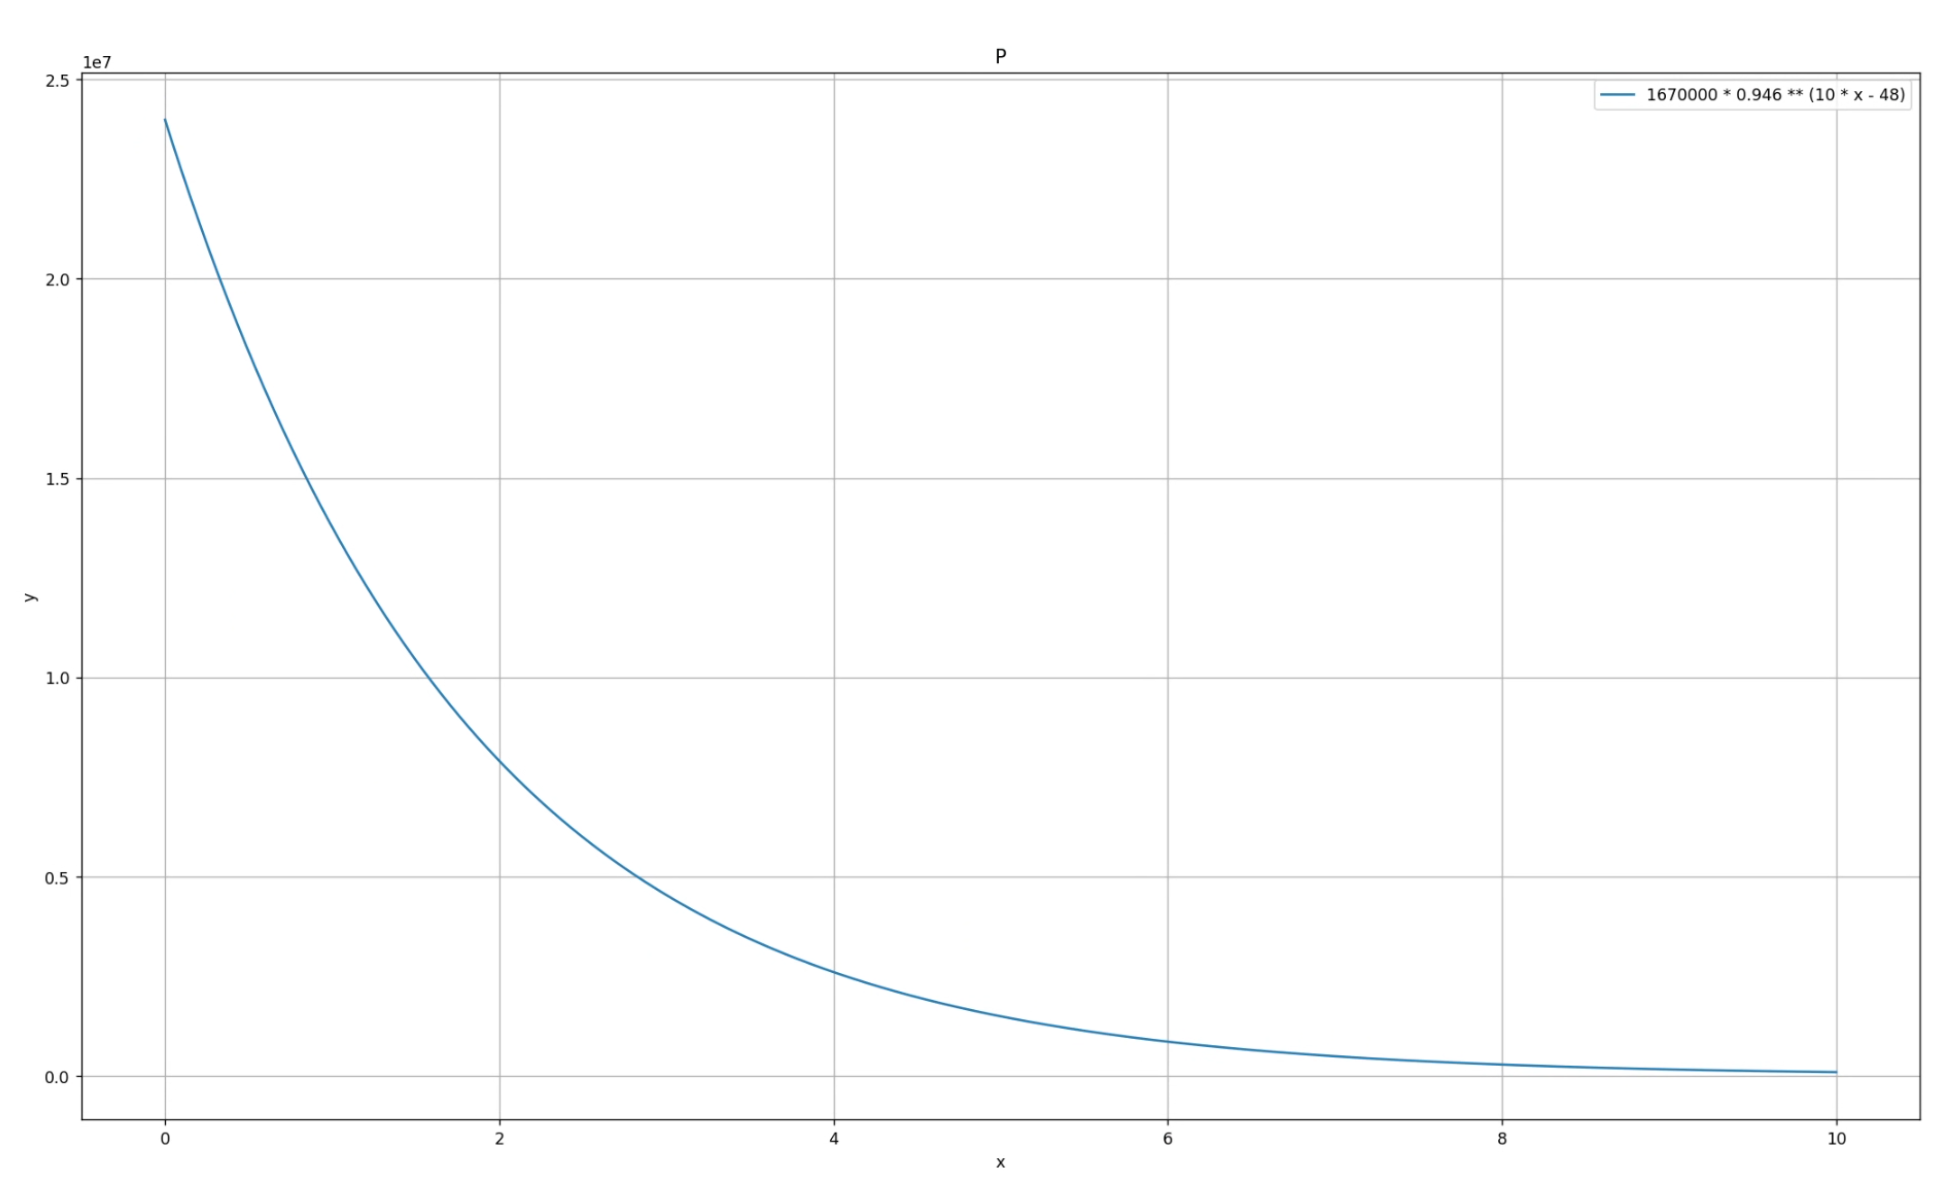
\includegraphics[width=1\textwidth]{model1.png} %图片的名称或者路径之中有空格会出问题 
    \caption{Relationship between Tourist Count and Tax Rate} % 图片标题                 
    \label{fig1}%交互引用
    \end{figure}
\item Mathematical model of tourist satisfaction\\
Through the causal model established earlier, we define that tourist satisfaction is calculated by CIS and CTS. For CIS, we define:
$$CIS=F(IS)$$
$$IS=CDI+TTI$$

The function F converts the State of infrastructures into the CIS function, which will be explained later. By consulting the government report \cite{Inf},we obtain the government's EIE and CDI. By fitting the data, we obtain the mathematical model of CDI:
$$
CDI=
\begin{cases}
    -12C^{1.05}, &if\ C\ is\ no\ more\ than\ 15000\\
    -12C^{1.06}, &if\ C\ is\ more\ than\ 15000
\end{cases}
$$
For the tax revenue, we can calculate it using E and x obtained from the report \cite{spend}:
$$T=C\cdot E\cdot x$$
Based on the data in the report and the expenditure on infrastructure in previous years, we have finally fitted the function of TTI.
$$TTI=
\begin{cases}
    T-150000, &if\ T\ is\ no\ more\ than\ 546000\\
    \frac{25T}{1.2 \log_{1.4}{100x}}, &if\ T\ is\ more\ than\ 546000
\end{cases}
$$
Its graph is as follows:
\begin{figure}[H]  %h此处,t页顶,b页底,p独立一页,浮动体出现的位置 [H]
 
    \centering  %图表居中
    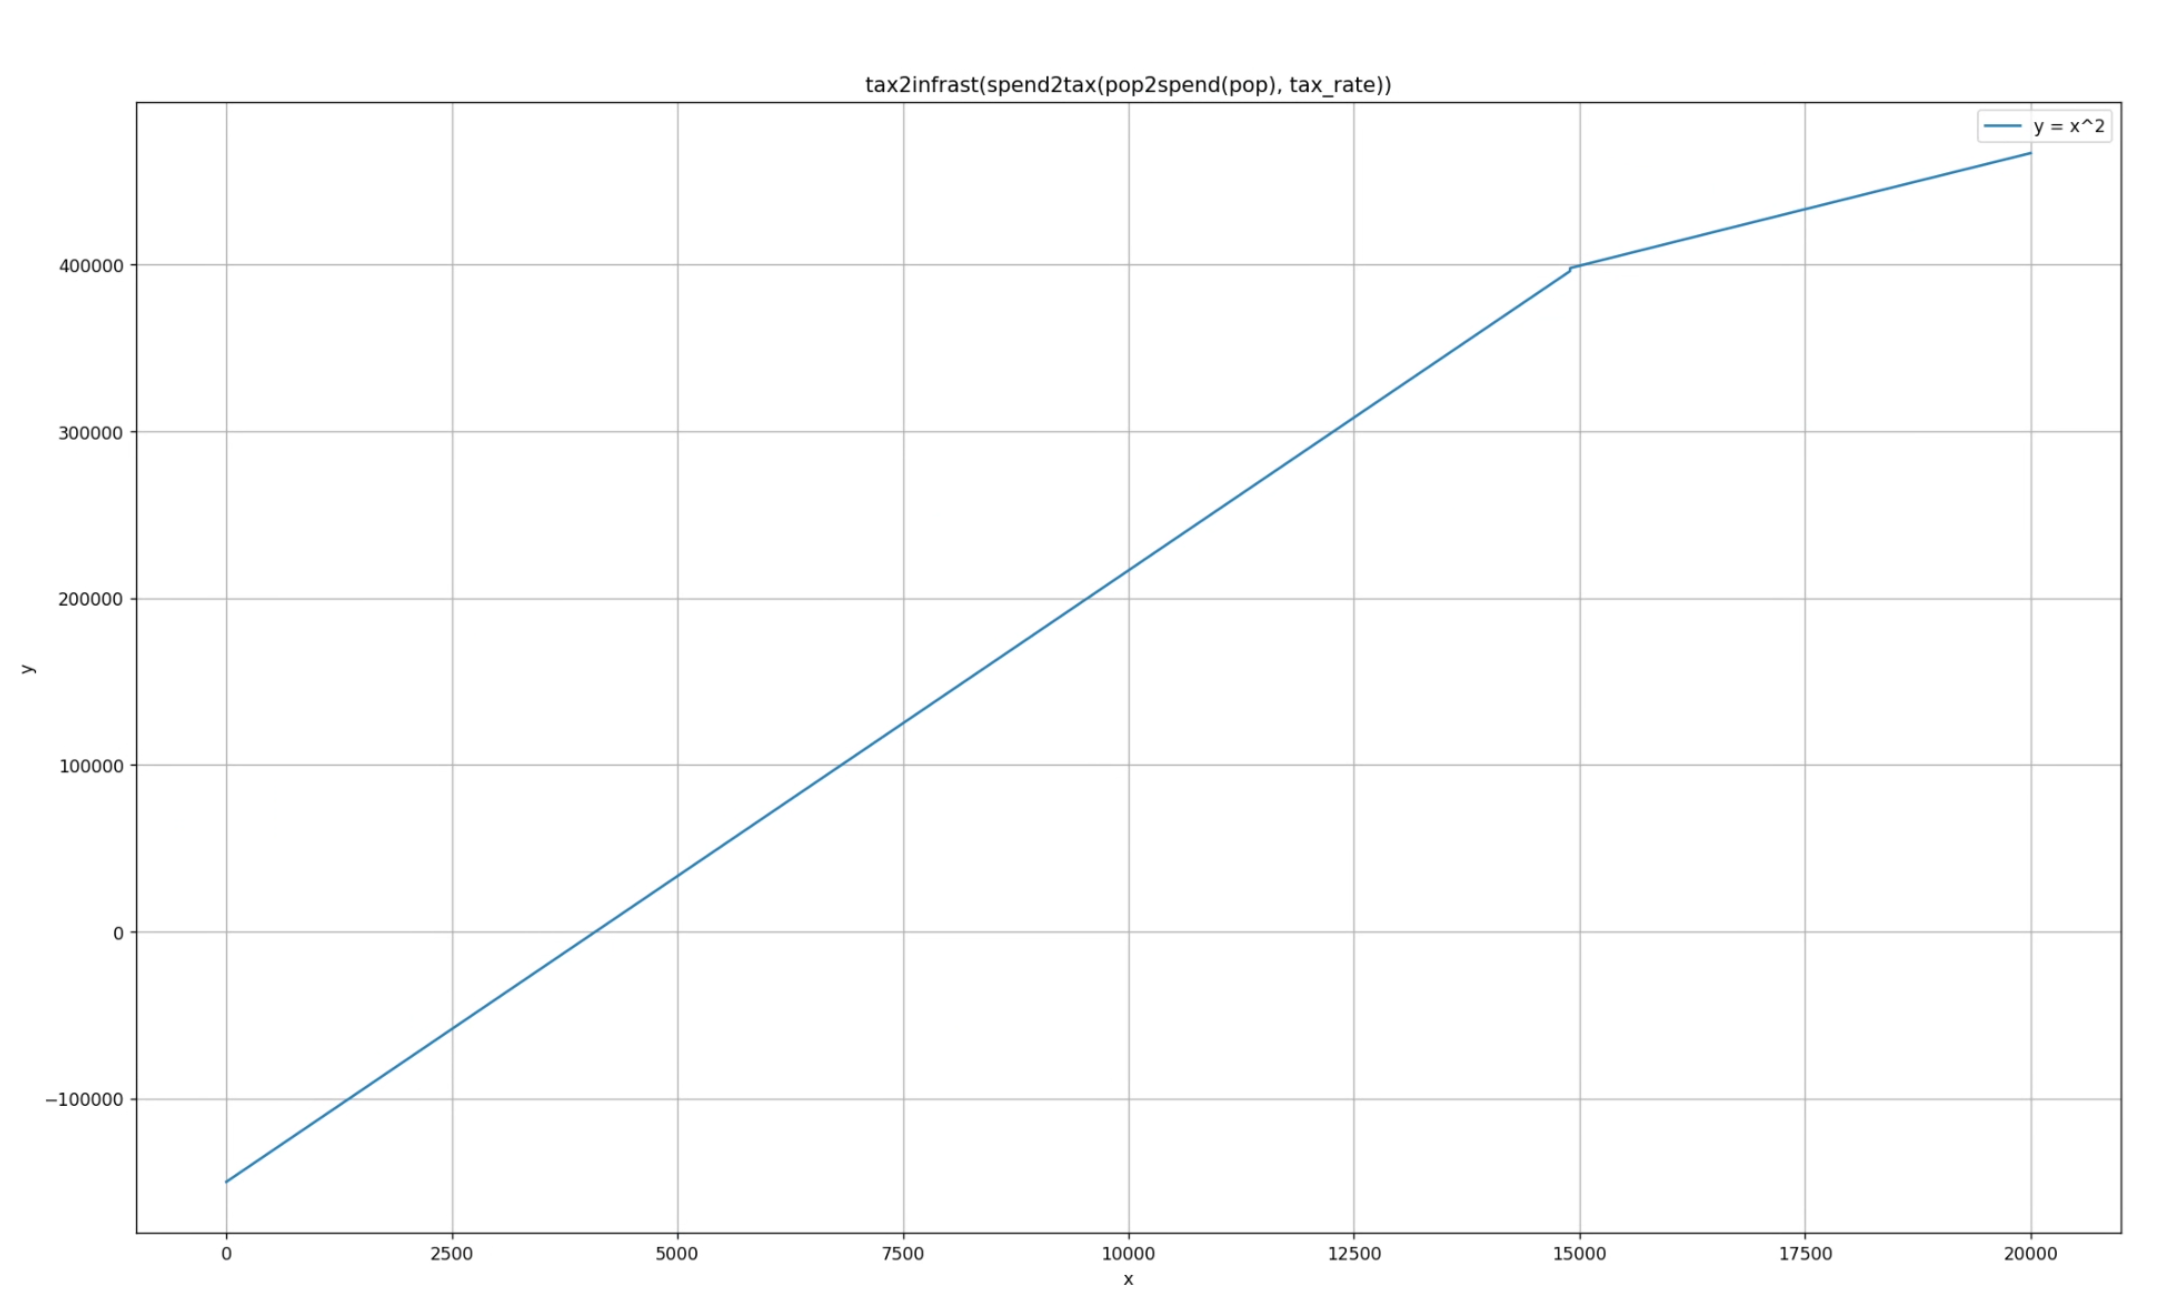
\includegraphics[width=0.9\textwidth]{tax2inf.png} %图片的名称或者路径之中有空格会出问题 
    \caption{Graph of TTI} % 图片标题                 
    \label{fig1}%交互引用
    \end{figure}
    The model shows that when the tax revenue invested in infrastructure increases to a certain extent, the input-output efficiency will decrease. Thus, we can obtain the graph of IS:
\begin{figure}[H]  %h此处,t页顶,b页底,p独立一页,浮动体出现的位置 [H]
 
    \centering  %图表居中
    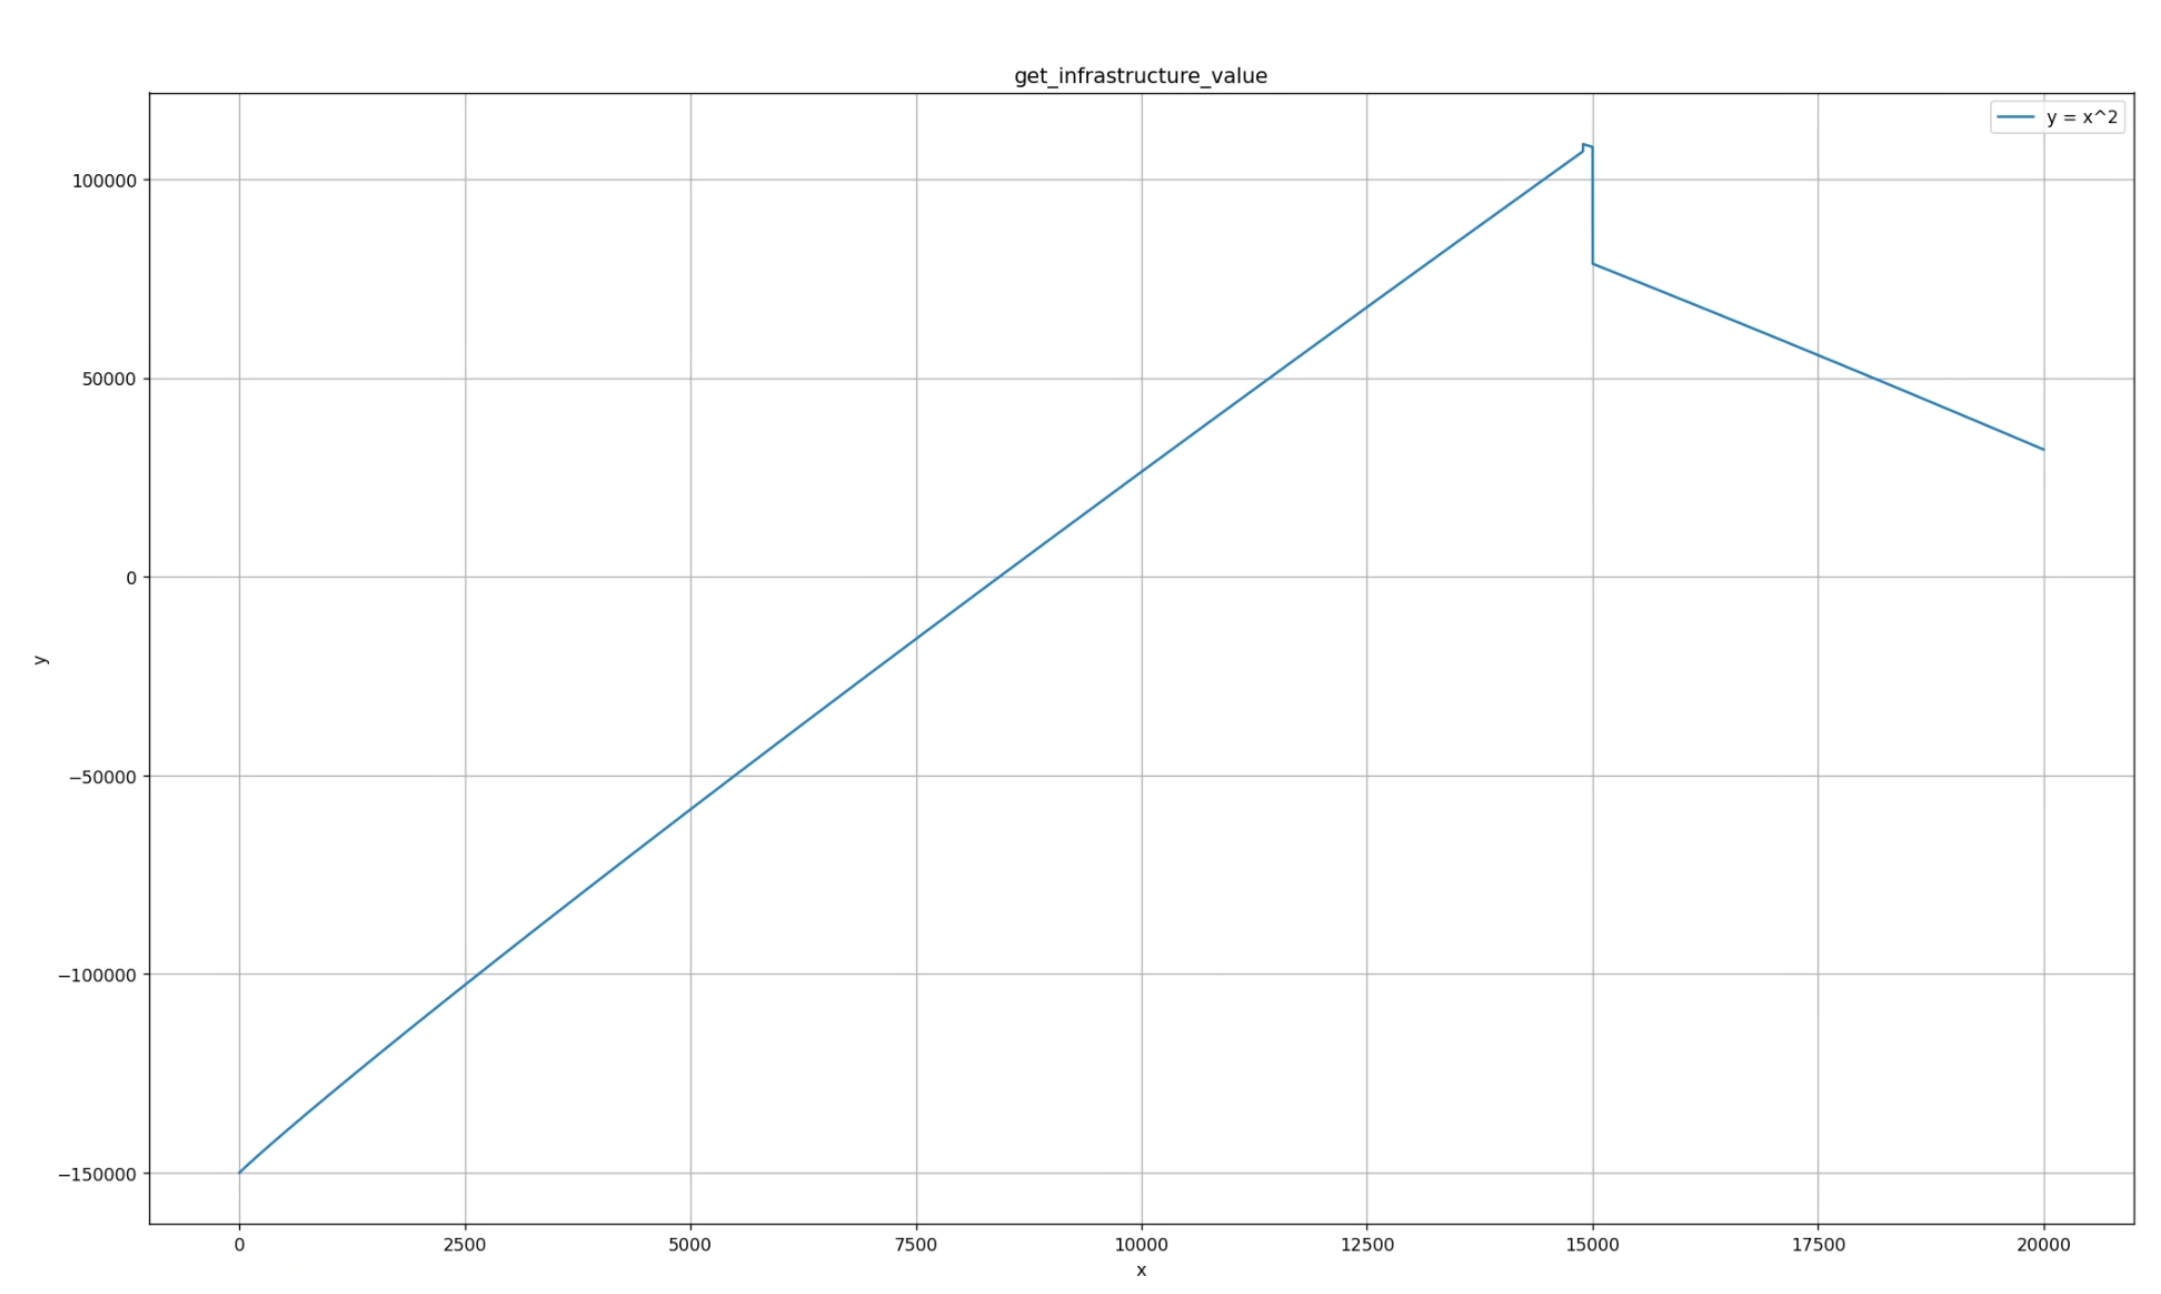
\includegraphics[width=0.9\textwidth]{IS.png} %图片的名称或者路径之中有空格会出问题 
    \caption{Graph of IS} % 图片标题                 
    \label{fig1}%交互引用
    \end{figure}
    F is the function that transforms IS into satisfaction, which is applicable to both locals and tourists. We define satisfaction as an evaluation metric with a value range of -100 to 100.
$$
CIS(LIS)=
\begin{cases}
    IS\times 2.408\times 10^{-5}-100, &if\ IS\ is\ no\ more\ than\ 4200000\\
    \log_{1.01}{\frac{x-10}{40000}}-470, &11624010\geq IS \geq 4200000
\end{cases}
$$
Finally, we get a function:
$$CS=U(CIS,CTS)$$
\item Mathematical model of locals' satisfaction

Similarly, we can divide the satisfaction of local residents (LS) into LinS and LIS. 

For Inc, we obtain the following mathematical model:
$$Inc=C\cdot E\cdot (1-x)\times \frac{365}{10000}$$
Where multiplying by 365 calculates the annual income. Given that Juneau has 30,000 residents and assuming each household consists of three people, we can obtain Inc. Based on the data from \cite{Hap} on income and happiness, we have fitted the curve:
$$LinS=
\begin{cases}
    (\log_{5}{\frac{\frac{Inc}{12}+6500}{480000}}+2.25)\times \frac{100}{0.4}\\
    (\log_{10}{\frac{Inc+400000}{480000}}+0.152)\times \frac{100}{0.4}
\end{cases}
$$
As for the LIS, the formula is the same as that for CIS, and will not be repeated here. Ultimately, we obtain the following function:
$$LS=U(LinS,LIS)$$
\item Glacier melting model\\
The calculation method for glacier melting speed can be obtained from the literature \cite{glac}:
$$THF=\frac{wTHF}{C}$$
$$GM=\alpha \cdot THF$$
Here, by substituting the data, we obtain the estimated glacier melting amount as $2.34×10−7 m/a/person$.
\end{enumerate}
 \section{Multi-Objective Optimization Model}
 \subsection{The Analytic Hierarchy Process}
 The Analytic Hierarchy Process(AHP) is a kind of method which combines qualitative and quantitative methods to calculate the decision weight of complex multi-objective problem. To figure out a comprehensive solution, we use AHP to estimate LS and CS.
 \begin{table}[H]
    \begin{center}
    \begin{tabular}{c|c}
    c1 & 0.98 \\
    c2 & 0.02 \\
    l1 & 0.5  \\
    l2 & 0.5 \\
    \end{tabular}
\end{center}
    \end{table}
    Then we can get LS and CS:\\
$$CS=c1\cdot CIS+c2\cdot CTS$$
$$LS=l1\cdot LinS+l2\cdot LIS$$
Now we can get exact numbers of CS and LS, to make further optimization, we will use NSGA-II algorithm to get a Pareto solution.
 \subsection{NSGA-II Processing}
 NSGA-II is a genetic algorithm used to solve multi-objective optimization problems. It iteratively finds the Pareto optimal solutions. Pareto optimal solutions may not be unique but rather a set of all optimal solutions. Pareto optimal solutions arise because the answers generated from the problem are non-dominated with respect to each other.
The steps of the algorithm are as follows:
1. Initialize the population: Randomly generate an initial population containing multiple individuals.

2. Calculate fitness: Calculate the fitness of each individual in the objective function space.

3. Non-dominated sorting: Divide the individuals in the population into multiple fronts to identify the different positions of individuals on the Pareto front.

4. Calculate crowding distance: Calculate the crowding distance to measure the density of individuals in the objective space.

5. Selection operation: Through binary selection operation, randomly select two individuals from the population and choose the individual with a higher non-domination level.

6. Crossover and mutation operations: Generate the parent population through crossover and mutation operations on the selected individuals, and combine the parent and offspring populations into a larger candidate population.

7. Iteration: Reapply the above steps to the candidate population until the stopping condition is met.

Here, we construct a multi-objective function and consider the reduction in tourists caused by glacier melting as a constraint condition at the same time:
 $$minf(C)=\{-CS(C),-LS(C)\}$$
 $$=
 13670.13\leq C\leq15211.08$$
 
 
 

 \section{Sensitivity Analysis}
 \subsection{CDI changes}
 
 
 \begin{figure}[H]  %h此处,t页顶,b页底,p独立一页,浮动体出现的位置 [H]
 
 \centering  %图表居中
 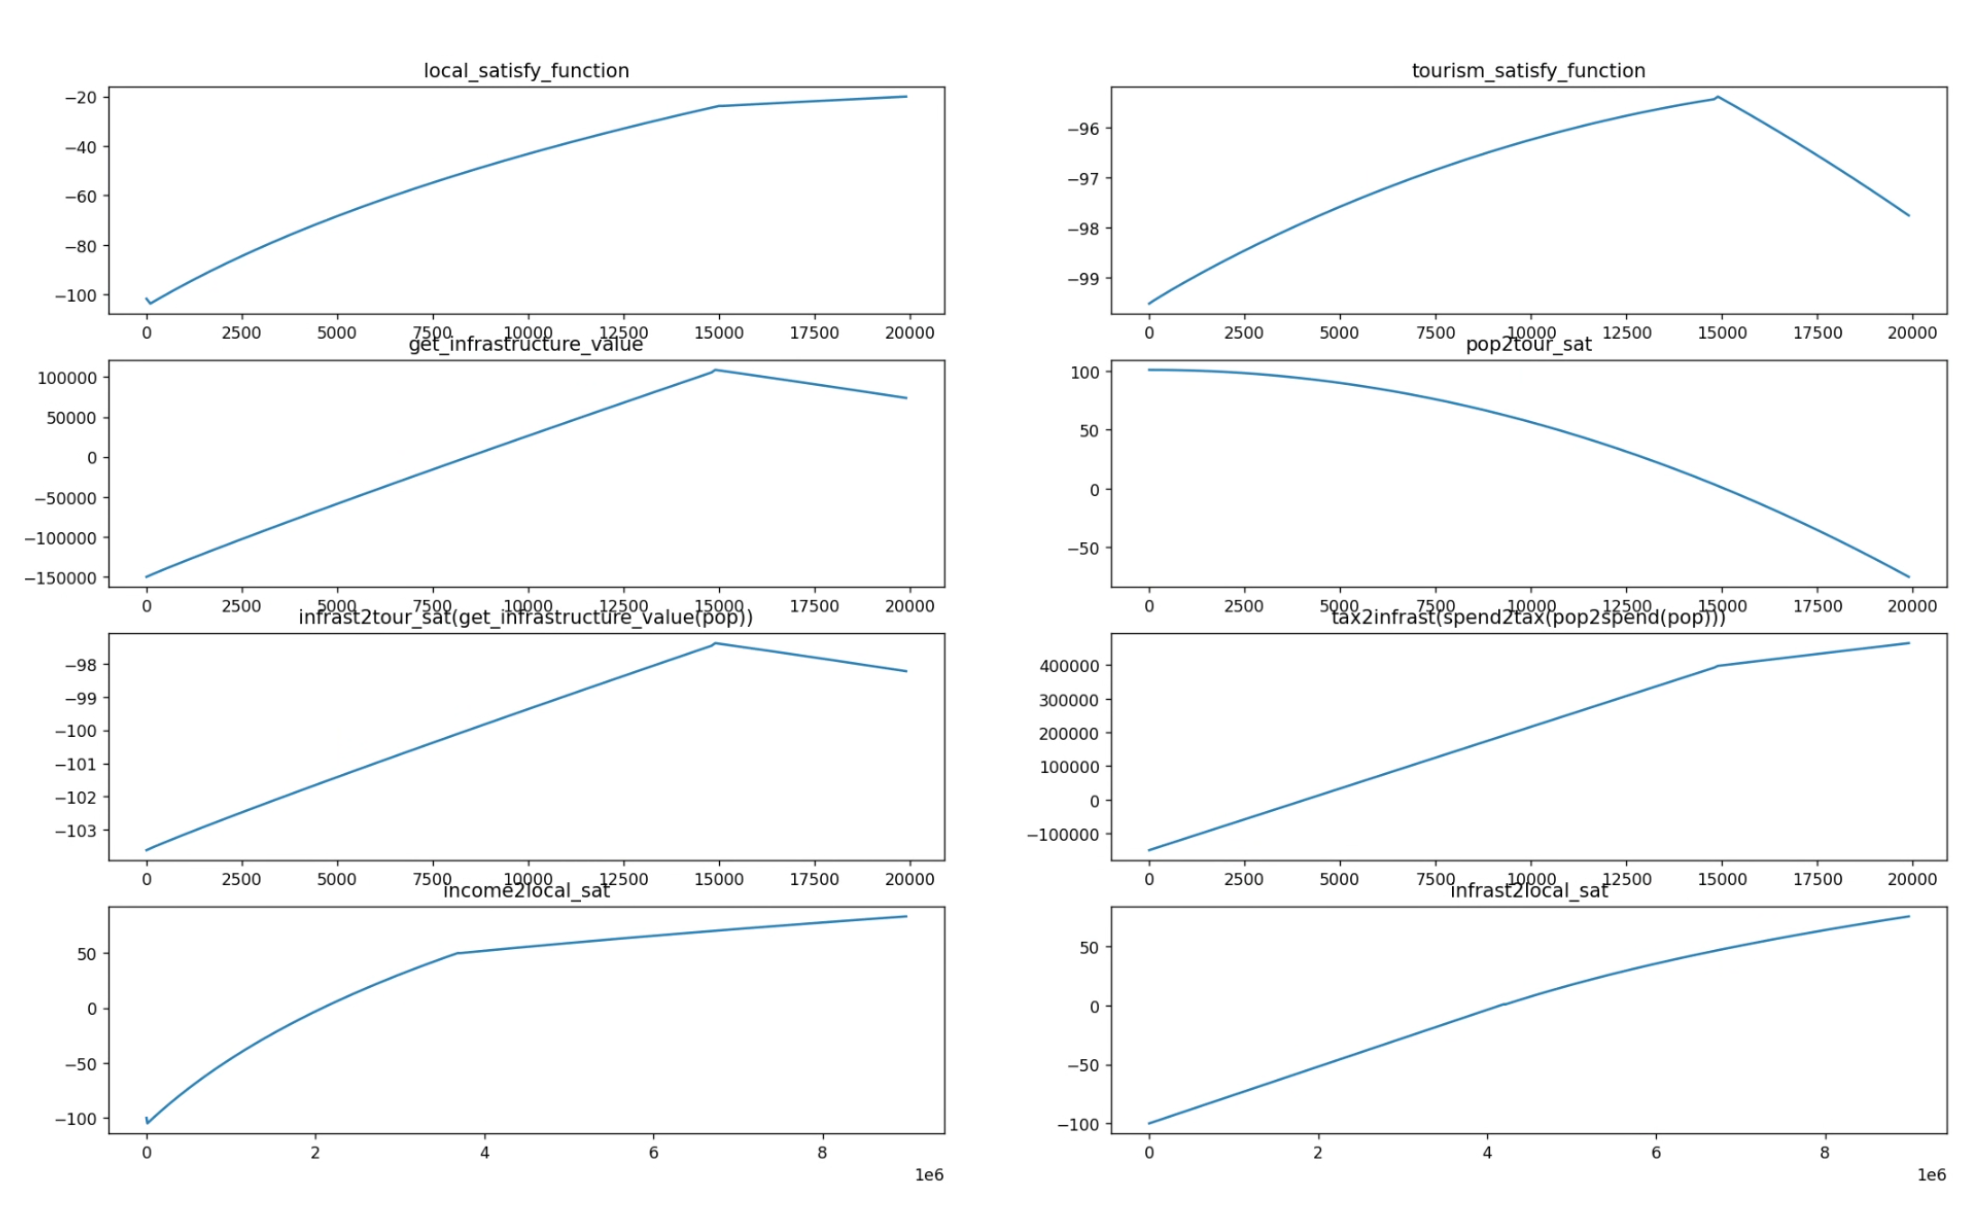
\includegraphics[width=.9\textwidth]{sensitivity12.png} %图片的名称或者路径之中有空格会出问题 
 \caption{The optimal tourist count at an infrastructure maintenance expense per tourist of \$8} % 图片标题                 
 \label{figx}%交互引用
 \end{figure}

 
 \begin{figure}[H]  %h此处,t页顶,b页底,p独立一页,浮动体出现的位置 [H]
 
 \centering  %图表居中
 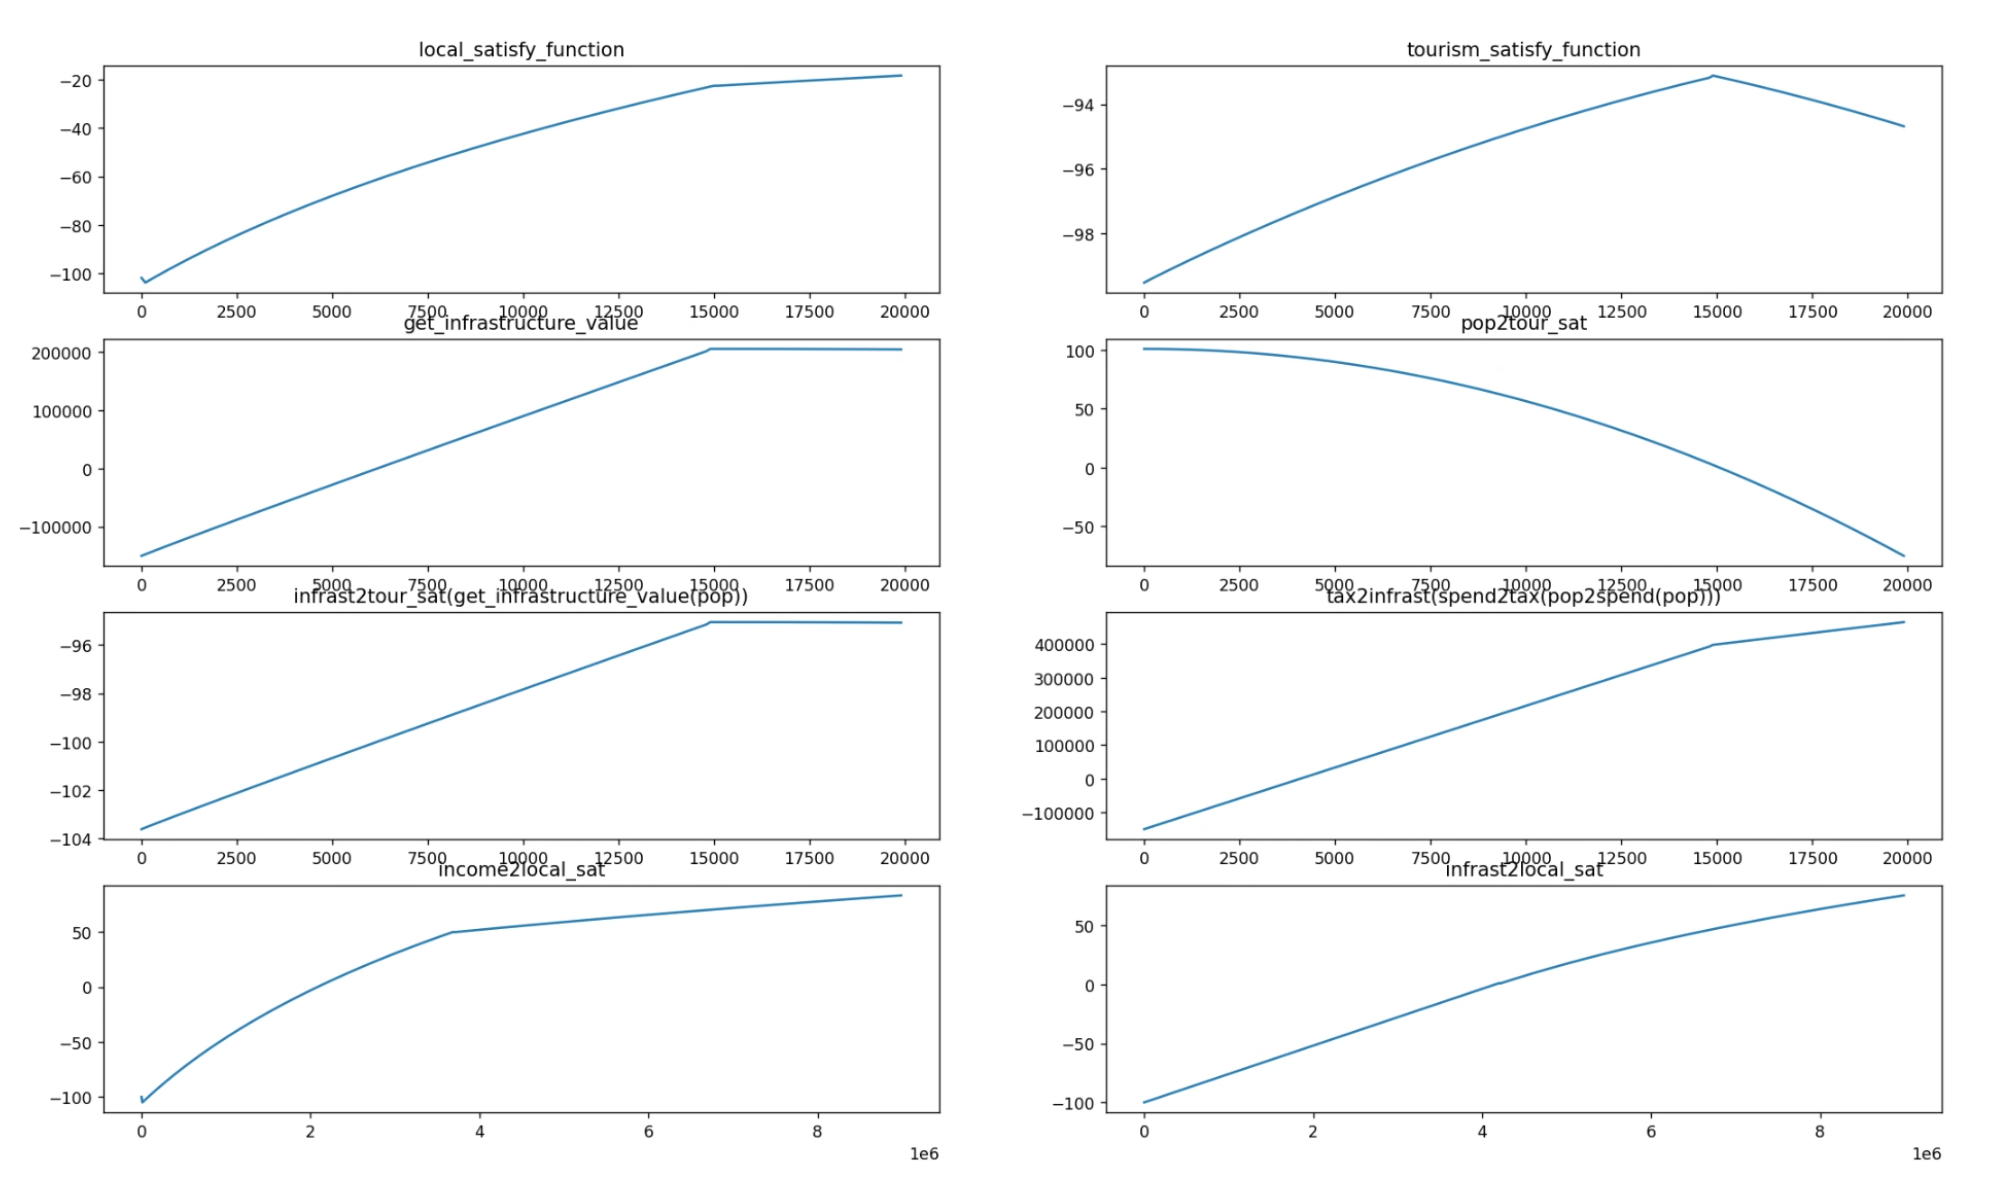
\includegraphics[width=.9\textwidth]{sensitivity8.png} %图片的名称或者路径之中有空格会出问题 
 \caption{The optimal tourist count at an infrastructure maintenance expense per tourist of \$8} % 图片标题                 
 \label{figy}%交互引用
 \end{figure}

 As shown in the figure, when CDI decreases from $12 to $8, the optimal tourist count does not change and remains around 15000,
 Therefore, it can be considered that the optimal tourist count is relatively insensitive to CDI and has strong robustness. 
 \subsection{Increase in tax rate}
  %我们把船票价格提升20\%,额外的收入用于维护旅游环境;结果显示,可持续旅游人数限制上升至15620人,表明额外的船税对维护可持续旅游有轻微积极影响;
    %我们提升了3\%的综合税率,结果显示,可持续旅游人数限制上升至16060人,表明额外的综合税率对维护可持续旅游有中度影响;但是,由于维护环境,特别是保护冰川的边际效益较小,更高的税率对提升可持续旅游人数限制不产生显著作用,反而可能减少游客的旅游意愿。
    We increased the ferry ticket price by 20\%, and allocated the additional revenue to the maintenance of the tourism environment; the results showed that the sustainable limit for the number of tourists increased to 15,620, indicating that the additional ferry tax has a slight positive effect on maintaining sustainable tourism.
    
    We raised the comprehensive tax rate by 3\%, and the results indicated that the sustainable limit for the number of tourists increased to 16,060, suggesting that the additional comprehensive tax rate has a moderate impact on maintaining sustainable tourism. However, due to the diminishing marginal benefits of environmental conservation, especially the protection of glaciers, higher tax rates do not significantly enhance the sustainable limit for the number of tourists and may instead reduce tourists' willingness to travel.
    \subsection{The reduction of environmental protection costs}
    Investing in environmental protection publicity advertisements may be beneficial for preserving the tourism environment. Based on the information provided, we assume that the government allocates a portion of its funds for publicity purposes, thereby reducing the costs needed to maintain the environment for each tourist. The results indicate that with just a 4\% increase in the ferry tax, the sustainable limit for the number of tourists rises to 16,620, showing that investing in environmental protection publicity advertisements has a significantly positive effect compared to direct investment in environmental protection, especially under moderate-scale promotion. Therefore, we recommend that the government invest in advertising campaigns to encourage tourists to protect the environment.
 
\section{模型迁移}
对于其他的地区,我们需要考虑用新的景区数据来进行约束。在这里我们定义:
$$A=V-kC$$
其中A是景区的吸引力,V是景区固有的价值,C依旧表示游客人数,k是描述旅游人数对景区的负面影响的常数。通过这个公式,只需要获取景区相应的数据进行计算便可得到最佳人数结果。\\
不仅如此,对于人数较少的景区,我们可以通过降低旅游税以获得更多的游客,该模型同样适用。对于人数爆满的景区,我们建议同时采用提高税收和限制旅游人数的方式来减少游客人数,这样能实现一个动态的平衡。
 \section{Strengths and weaknesses}
 
 \subsection{Strengths}
 
 \begin{itemize}
     \setlength{\parsep}{0ex} %段落间距
     \setlength{\topsep}{2ex} %列表到上下文的垂直距离
     \setlength{\itemsep}{1ex} %条目间距
     \item In the causal model, the impact of the number of tourists on residents' income, government revenue, infrastructure conditions, and the ecological environment has been fully taken into account.
     \item The appropriately modified model can be applied to another destination affected by over-tourism, demonstrating its versatility.
     \item When solving the multi-objective optimization problem, the NSGA-II genetic algorithm was employed, which integrates neural networks and symbolic reasoning, and is characterized by its robustness.
 \end{itemize}
 
 \subsection{Weaknesses}

 \begin{itemize}
    \setlength{\parsep}{0ex} %段落间距
     \setlength{\topsep}{2ex} %列表到上下文的垂直距离
     \setlength{\itemsep}{1ex} %条目间距
      \item The effect of sudden natural disasters on Juneau's tourism industry was not considered.
      \item The algorithm did not incorporate the conservation of tourism resources beyond glaciers as a constraint.
      \item The algorithm did not take into account how the allocation ratio of government funding for environmental protection and infrastructure maintenance changes with the total tax revenue.
 \end{itemize}
 
 
 \clearpage
 %另起一页继续写。这时,你最好使用“\clearpage” 
 \section{A Memo to the tourist council of Juneau}
 \noindent
 \textbf{Date:} January 27th, 2025

 \noindent
 \textbf{To:} Tourist Council of Juneau

 \noindent
 \textbf{From:} MCM Team \#2511654

 \noindent
 \textbf{Subject: A Multi-Objective Optimization Model for Adjusting Tourist Count}
 {\noindent}	 \rule[-0pt]{16.5cm}{0.15em}\\
\noindent
\textbf{Dear members of the council:}

As tourism flourishes in Juneau, we recognize that over-tourism may bring challenges to our city. To promote economic development while protecting our natural environment and residents' quality of life, our team has conducted in-depth research and developed a comprehensive and reliable model, yielding practical predictions and recommendations.

\noindent
\textbf{Our Model and Advantages}

\textbf{1. Comprehensive Causal Model:} We have created a comprehensive causal model that analyzes the impact of tourist numbers on residents' income, government revenue, infrastructure conditions, and the ecological environment. Based on reliable data, we have conducted mathematical modeling to provide a holistic understanding of the interplay between tourism and various aspects of our city.

\textbf{2. Reliable Multi-Objective Optimization Model:} We have established reliable functions for tourist and resident satisfaction and used genetic algorithms to obtain the Pareto solution for tourist numbers, maximizing the satisfaction of all stakeholders.

\noindent
\textbf{Our Predictions}

After solving the multi-objective optimization model, we recommend maintaining the current tourist numbers at around 14,550 to promote sustainable tourism.

\noindent
\textbf{Our Recommendations}

\textbf{1. Gradual Tax Increase: }A gradual increase in taxes (ranging from 3\% to 20\%) will help raise the tourist limit necessary for sustainable tourism development.

\textbf{2. Environmental Protection Campaign: }Allocating a portion of the funds to launch environmental protection campaigns and encouraging tourists to protect the environment can reduce the economic costs associated with environmental protection.

We believe implementing these measures will balance tourism development and environmental protection, ensuring a sustainable future for Juneau.

\noindent Sincerely,

\noindent Team \#2511654
%针对朱诺市过度旅游的现状,我将向您展示我们的模型优势和预测结果,并提出措施建议。
%
%·我们的模型和优势:
%1.考虑因素全面的因果模型:我们综合分析了游客人数对居民收入、政府税收、基础设施状态和生态环境的影响,根据可靠数据进行数学建模
%.结果可靠的多目标优化模型:我们建立可靠的游客满意度和居民满意度函数,运用遗传算法求得游客数量的Pareto解,最大化利益相关方的满意度

%·我们得出的预测结果:
%经过求解多目标优化模型,我们推荐在当前状态下,控制旅游人数在14550人左右,以推进可持续旅游

%·我们的建议措施:
%1.适度提升税率(提升范围在3\%至20\%)有利于提高维持旅游业可持续发展的游客限额
%2.支出部分款项用于投放保护环境的宣传广告,倡议游客保护环境,能降低投入环境保护的经济成本
 % 参考文献,务必统一格式,下面以书籍、期刊文章、网页资料为例
 \clearpage   %另起一页继续写。这时,你最好使用“\clearpage” 
 
 \begin{thebibliography}{99}
    \bibitem{taxandtour}
    Adedoyin, F. F., Seetaram, N., Disegna, M., \& Filis, G. (2023). The Effect of Tourism Taxation on International Arrivals to a Small Tourism-Dependent Economy. Journal of Travel Research, 62(1), 135-153. 
     
    \bibitem{pop}
    Formery McDowell Croup, ECONOMIC IMPACT OF JUNEAU\textquotesingle S CRUISE INDUSTRY 2023
    {https://juneau.org/wp-content/uploads/2024/01/CBJ-Cruise-Impacts-2023-Report-1.22.24.pdf}

    \bibitem{spend}
    Juneau Tourism Survey 2023 \& Juneau Cruise Passenger Survey 2023 \& Juneau Cruise Industry Impacts 2023 Extended Slide Deck, McKINLEY RESEARCH
    {https://www.seconference.org/wp-content/uploads/2024/02/Tourism-Panel-Heather-Haugland.pdf}

    \bibitem{Inf}
    Biennial Budget of Juneau \href{https://juneau.org/wp-content/uploads/2024/08/FY25-Adopted-Budget-Book-Final.pdf}{https://juneau.org/wp-content/uploads/2024/08/FY25-Adopted-Budget-Book-Final.pdf}

   \bibitem{Hap}
   Income and Happiness \href{https://osf.io/cfnbv}{https://osf.io/cfnbv}

   \bibitem{glac}
    Shuxin Wang, Jiankuo Du, Shuang Li, Hong He, Wei Xu:
    Impact of tourism activities on glacial changes based on the tourism heat footprint (THF) method,Journal of Cleaner Production, 215, 845--853, (2019).
   
 \end{thebibliography}
 
 % \includepdf[pages={1,2}]{Memo.pdf} 
 
 \end{document}  % 结束